%%%% CAPÍTULO 2 - REVISÃO DA LITERATURA (OU REVISÃO BIBLIOGRÁFICA, ESTADO DA ARTE, ESTADO DO CONHECIMENTO)
%%
%% O autor deve registrar seu conhecimento sobre a
%% literatura básica do assunto, discutindo e 
%% comentando a informação já publicada. A revisão deve
%% ser apresentada, preferencialmente, em ordem
%% cronológica e por blocos de assunto, procurando
%% mostrar a evolução do tema.

%% Título e rótulo de capítulo (rótulos não devem conter caracteres especiais, acentuados ou cedilha)
\chapter{Fundamentação teórica e trabalhos correlatos}
\label{cap:revisaodaliteratura}
%\chapter{Revisão da Literatura}\label{cap:revisaodaliteratura}



\section{Grafos} \label{sec:grafos}

A  Figura~\ref{fig:graphtheory}

 \begin{figure}[!h]
 \caption{Origem da teoria dos grafos}
     \centering
     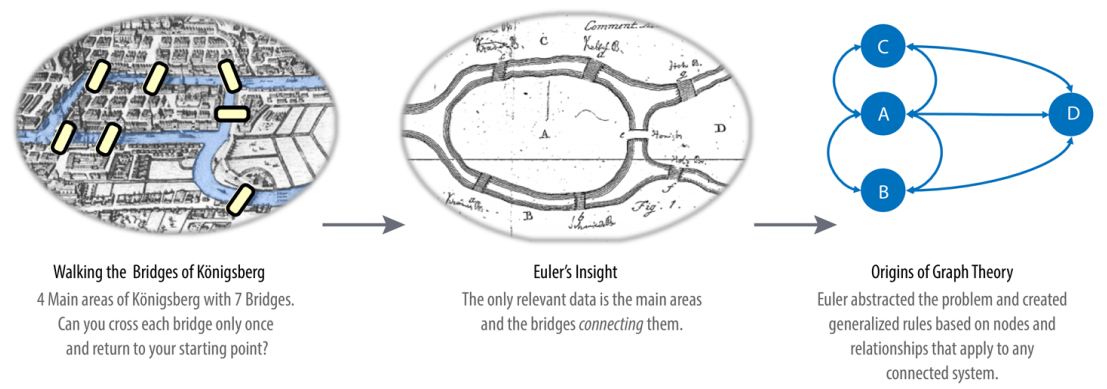
\includegraphics[scale=.40]{./Capitulo2/img/origins-graph-theory.png}
         \label{fig:graphtheory}
     \fonte{\cite{needham:2019}}
 \end{figure}
 
 
\section{Time Varying Graph (TVG)} \label{sec:tvg}

%Referências:\\
%\cite{hol:12} (Mais geral sobre Temporal Networks; Samaki tem )\\
%\cite{lat:10} (Menciona TVGs como uma sequência de grafos)\\
%\cite{sant:12} (TVG basico)\\
%\cite{cat:13} (TVG e Neo4j)\\
%\cite{lat:12} (TVG)\\
%\cite{wach:17} (People in Motion Lab)\\
%\cite{wach:19} (People in Motion Lab)\\
%\cite{vick:10} (Comparação Graph and Relational Database)
\textcolor{courb2020}{
O termo \emph{Time Varying Graph} (grafo variante no tempo ou TVG) pode ser encontrado em \cite{sant:09}, \cite{tang:10}, \cite{lat:10} e \cite{lat:12}. O formalismo adotado no presente trabalho é devido a~\cite{sant:12}. 
}
\textcolor{courb2020}{
Um TVG é uma quíntupla $\mathcal{G}=(V,E,\mathcal{T},\rho,\zeta)$, tal que $V$ e $E$ são os conjuntos de vértices e arestas do grafo rotuladas pelo conjunto $L$ de rótulos ($E \subseteq V \times V \times L$), respectivamente, $\mathcal{T}\subseteq \mathbb{T}$ é o tempo de vida do sistema, $\rho: E \times \mathcal{T} \rightarrow \{0,1\}$ é a função de presença e $\zeta: E \times \mathcal{T} \rightarrow \mathbb{T}$ é a função de latência. O domínio temporal $\mathbb{T}$ é assumido igual a $\mathbb{N}$ para sistemas a tempo discreto e $\mathbb{R}^+$ para para sistemas a tempo contínuo.
}
\textcolor{courb2020}{
A função $\rho$ indica a presença (1) ou não (0) de uma aresta em um determinado instante de tempo e a função $\zeta$ representa o tempo necessário para cruzar uma aresta a partir de um determinado instante de tempo (a latência pode variar com o tempo). Este modelo é geral o suficiente para representar vários cenários, desde redes de comunicação e transporte até sistemas complexos ou redes sociais~\cite{sant:12}. 
}
\textcolor{courb2020}{
Por exemplo, um TVG pode ser usado para modelar viagens de uma cidade $A$ para uma cidade $B$. As cidades $A$ e $B$ são os vértices do grafo conectados por duas arestas paralelas rotuladas `ônibus' e `carro' para indicar viagens feitas de ônibus e de carro, respectivamente. Neste caso, a viagem de ônibus inicia em instantes de tempo determinados e, portanto, a função $\rho$ da aresta `ônibus' retorna valor 1 apenas nas datas e horários para os quais a viagem de ônibus pode ser iniciada. A função de latência $\zeta$ de cada aresta  pode retornar diferentes valores, dependendo dos tempos de viagem de ônibus e de carro (ou mesmo diferentes valores para uma mesma aresta, dependendo do tempo de viagem em diferentes horários).
}
\textcolor{courb2020}{
A partir deste modelo geral de~\cite{sant:12}, um modelo de dados é proposto em \cite{cat:13} para capturar o comportamento temporal de redes sociais e implementado no banco de dados de grafos Neo4j. O banco Neo4j implementa um tipo de grafo denominado \emph{property graph model}, capaz de representar multigrafos direcionados, rotulados e com atributos. Estes grafos permitem a representação de vértices e arestas rotulados, além de metadados (propriedades) associados aos vértices e arestas~\cite{rod:10}, particularmente importantes na implementação de TVGs. Além disso, o banco de dados Neo4j tem outras características que favorecem a implementação: (i) armazenamento persistente e transacional de grafos de elevada dimensão; suporte para análise em profundidade via buscas eficientes de múltiplos saltos; (iii) suporte para linguagem declarativa de \emph{queries} de grafos denominada Cypher\footnote{https://neo4j.com/docs/cypher-manual/current/}.
}
\textcolor{courb2020}{
O modelo proposto para o transporte público de Curitiba tem por base o modelo de grafo utilizado em \cite{wach:19} para o transporte de ônibus da região de Greater Moncton no Canadá. Este modelo deriva de~\cite{cat:13}, tendo sido também implementado no banco Neo4j.
}

\section{Métricas de Redes Complexas} \label{sec:metr}


Uma vez que o grafo do sistema de transporte descrito na seção anterior é modelado e armazenado no Neo4j, métricas de redes complexas podem ser computadas para avaliar o comportamento do sistema. 
Tais métricas permitem uma avaliação da importância dos vértices na rede (pontos de ônibus), tanto do ponto de vista estático da topologia da rede quanto dinâmico da movimentação dos ônibus, e sua relação com os outros pontos da rede.
Esta seção descreve as métricas utilizadas neste trabalho: 

\subsection{Centralidade de grau}


Proposto por~\cite{free:79}, a centralidade de grau é proporcional ao número de arestas (de entrada, ou de saída em grafos direcionados) que se conectam a um determinado vértice. Quanto maior a centralidade de grau de um vértice, maior é o número de conexões com outros vértices.

No caso da rede de transporte, na perspectiva de dinamicidade da rede através da interatividade de veículos com seus respectivos pontos de ônibus, a centralidade de grau de um vértice \emph{BusStop} é proporcional ao número de paradas de ônibus no respectivo ponto. Isso pode significar que pontos com elevada centralidade de grau podem corresponder a locais de potencial congestionamento ou de formação de comboios decorrente de uma estratégia de atendimento de demanda elevada. 

Na perspectiva da rede estática, isto é, isolando-se somente os pontos de ônibus e suas conexões, a centralidade de grau de um vértice \emph{BusStop} é proporcional ao número de linhas de ônibus que passam pelo vértice, já que apenas arestas para outros vértices \emph{BusStop} são consideradas. Um ponto ponto de ônibus com grande número de conexões apresenta uma grande oferta de linhas.

\subsection{Centralidade de intermediação}


Introduzido por \cite{free:77} como uma medida para quantificar o controle de um ser humano sobre a comunicação entre outros seres humanos em uma rede social, a centralidade de intermediação (\emph{betweenness centrality}) quantifica quão importante um vértice (ou uma aresta) é na definição dos caminhos possíveis entre vários (ou todos) os pares de vértices de uma rede. Isso permite calcular qual a capacidade da rede se ``recuperar'' em caso de remoção de um ou mais vértices. Também é importante, pois auxilia na identificação de vértices que atuam como ``intermediários de serviços'' na rede.

Em outras palavras, a remoção de vértices com elevada centralidade de intermediação podem degradar ou mesmo interromper o fluxo de informação em uma rede. 

Para um vértice, a centralidade de intermediação é definida pela proporção dos caminhos que empregam um determinado vértice em relação a todos os caminhos existentes, ou seja:

 \begin{equation}
     B(u) = \sum_{s \neq u \neq t }^{} p(u) / p,
 \end{equation} 
na qual:

 \begin{itemize}
 \item $u$: é um vértice.
 \item $p$: é o número total de caminhos entre os vértices $s$ e $t$.
 \item $p(u)$: é o número de caminhos entre os vértices $s$ e $t$ que passam pelo vértice $u$.
\end{itemize}  

No contexto de sistemas de transporte, vértices com significativo $B$ são potenciais pontos de estrangulamento do sistema, dada a dependência que os caminhos possíveis desse sistema têm desse vértice. Essa dependência pode ser temporal (ocorre em um intervalo de tempo específico) ou espacial (depende da posição espacial do ponto de ônibus), de acordo com o contexto de análise.

\subsection{Page rank}


O page rank foi concebido com o intuito de ranquear páginas (\emph{web sites}) relevantes da \emph{World Wide Web}. 

Usando o conceito presente em cadeias de Markov e/ou difusão em redes complexas, pode-se determinar os vértices mais significativos do ponto de vista de fluxos existentes em uma rede, quando o regime estacionário é atingido. Pode-se traduzir esse regime estacionário como a tendência de um usuário aleatório sempre chegar em uma determinada página, ou os dados em redes de comunicação sempre trafegarem por um determinado roteador.

A ideia é que o fluxo de navegação dos usuários defina a relevância das páginas ao reforçar suas interconexões (\emph{hyperlinks}). O algoritmo PageRank \cite{brin:98} traduz a ideia intuitiva de que usuários em geral tendem a acessar páginas e navegar pela WWW usando \emph{hiperlinks} até uma certa profundidade. Assim, páginas bem posicionadas no fluxo de navegação são relevantes, pois tendem a ser muito visitadas pelos usuários. 
No contexto das redes de transporte, um ponto de ônibus com elevado \emph{page rank} pode indicar conexões com outros pontos importantes. Por exemplo, ligações diretas entre terminais de ônibus no caso estático.


\subsection{Caminho mínimo}

O caminho mínimo entre dois vértices é o caminho com o menor número de arestas, no caso de arestas não ponderadas. 
Define-se caminho entre dois vértices quaisquer como a sequência de vértices, ligados dois a dois por arestas, que deve ser percorrida para conectá-los. As arestas podem ser ponderadas ou não, definindo características das ligações entre dois vértice e afetando a definição do caminho. A partir dos caminhos existentes entre dois nós quaisquer, define-se como caminho mais curto aquele cujo ``esforço'' exigido para percorrê-lo é o menor dentre os caminhos existentes.

Caso as arestas sejam ponderadas, deve-se considerar a soma dos pesos das arestas do caminho de um vértice a outro. A determinação de caminhos mínimos (considerando todos os pares de vértices de uma rede) é informação significativa para o planejamento urbano e a operação de um sistema de transporte, pois pode induzir no fluxo de pessoas na cidade. Algoritmos de caminho mínimo identificam rotas de conexão entre dois pontos da cidade de forma a minimizar o tempo de percurso necessário no transporte público \cite{Mart:2009, Larson:81}. Uma vez conhecidos os caminhos mínimos de todos os vértices para todos os outros da rede, define-se o diâmetro da rede como o caminho mínimo mais longo da rede.

% \subsection{Conectividade}

% \textcolor{courb2020}{
% Conectividade é um propriedade que indica existe pelo menos um caminho entre todos os pares de vértices de uma rede. Caso não haja, existem sub-grafos isolados dentro da rede.
% No contexto das redes TVGs aplicadas ao sistema de transporte público, a evolução temporal desse sistema pode ou não gerar intervalos de tempo nos quais parte da rede perde conectividade com o restante da rede. Essa mudança na conectividade da rede pode ser um comportamento estrutural (ou seja, é um fenômeno recorrente da rede) ou uma anomalia (um fenômeno aleatório, como um acidente que bloqueie a passagem de veículos por uma via pública).
% }

\subsection{Diâmetro e densidade de rede}

A partir do resultado do cálculo de caminhos e caminhos mínimos pode ser identificado o diâmetro (geodésico) de uma rede. O diâmetro de uma rede é o caminho mínimo mais longo dessa rede, ou seja, a distância entre dois vértices cujo caminho mínimo é o mais longo a ser percorrido. 

Naturalmente, o contexto de análise pode implicar que o diâmetro possa ser calculado a partir de atributos dos vértices e/ou arestas, como tempo exigido para percorrer dada par de vértice conectado, ou a distância entre esses pares de vértices conectados.
A densidade da rede mede a similaridade entre a rede e um grafo completo (grafo em que há um aresta para todos os seus pares de vértices) e pode ser definida como:

 \begin{equation}
     D = \mid E \mid / \mid N \mid ( \mid N \mid -1),
 \end{equation} 
na qual:

 \begin{itemize}
 \item $N$: é o número total de vértices.
 \item $E$: é o número total de arestas.
\end{itemize}  

\section{Trabalhos correlatos} \label{sec:fund}

\textcolor{courb2020}{
Para análise de desempenho da operação do transporte, é necessário incluir informação de tempo no modelo de rede utilizado. Em \cite{hol:12}, uma variedade de termos é apresentada para designar redes cuja estrutura é dependente do tempo: \emph{temporal graphs}, \emph{evolving graphs}, \emph{time-varying graphs}, \emph{time-aggregated graphs}, \emph{time-stamped graphs}, \emph{dynamic networks}, \emph{dynamic graphs}, \emph{dynamical graphs}, entre outros. O objetivo aqui não é discutir estes termos em profundidade, mas apenas destacar a ampla gama de opções para modelagem de redes dinâmicas. Particularmente, o modelo \emph{Time Varying Graph} (TVG) é adotado neste trabalho, tendo sido usado em \cite{sant:09}, além de \cite{tang:10} e \cite{lat:10} como uma sequência discreta e ordenada de grafos (a forma mais intuitiva de representação de um grafo variante no tempo). Um extensão dos conceitos clássicos de grafos para TVGs é apresentada em \cite{lat:12}. Em \cite{wach:19}, é apresentado um modelo TVG do transporte de ônibus de Greater Moncton no Canadá e sua implementação no banco de dados de grafos Neo4j\footnote{http://neo4j.org}. Conforme apontado em \cite{vick:10}, há um interesse crescente em bancos de dados noSQL (\emph{not only} SQL), como o Neo4j, para armazenamento e recuperação de dados com informação dinâmica.
}

\ric{O texto abaixo foi retirado de uma proposta de doutorado - precisa ver o que se aplica aqui e alterar o texto; já inclui as referências.}

Diversas aplicações em mobilidade urbana desenvolvidas a partir de modelos obtidos com o uso intensivo de dados podem ser encontradas em~\cite{Rosa2020}.

O estudo e análise de sistemas de transportes é imprescindível para o melhoramento do planejamento urbano e aperfeiçoamento da logística e processos pertencentes a estes sistemas em cidades inteligentes.
Em \cite{bon:16} por meio da aplicação da teoria de redes complexas foi possível analisar a topologia do sistema de transporte de ônibus em Curitiba e identificar características geográficas e espaciais. Foram utilizadas propriedades estáticas do sistema de transporte onde as paradas de ônibus formaram os nós e as arestas representaram as ligações entre os ônibus na construção da rede complexa. Foram aplicadas métricas como \emph{closeness centrality} que determina através de modelo matemático a proximidade de um nó em relação aos outros. A métrica \emph{betweenness centrality} define a importância de determinado nó dentro da rede. A partir dos resultados obtidos com a aplicação dessas métricas e outros conceitos foi possível realizar uma análise comparativa com estudos de outras cidades. Os resultados mostram os possíveis impactos que toda a rede pode sofrer com eventuais problemas nos terminais, além de demonstrar sugestões referentes à integração de pontos de embarque e desembarque para melhoria de qualidade nos serviços e aperfeiçoamento deste tipo de sistema. Em \cite{bart:15} foi realizada uma revisão apresentando os principais modelos de redes espaciais, onde um grafo possui vértices associados a posições no espaço geográfico, notadamente para redes de transporte. Estas análises foram feitas para redes estáticas.

Em \cite{gal:15} foram utilizados conceitos de redes multicamadas por meio de um \emp{framework} aplicado à rede de transporte do Reino Unido. Todos os modais de transporte públicos foram incluídos e cada modal foi atribuído a uma camada. Para cada conexão entre vértices, uma aresta ponderada com possíveis eventos foi modelada segundo horários de chegada e partida. Estes dados de horários integrados dos modais de transporte permitiram a construção de grafos temporais e redes multicamadas para a análise de características espaciais e temporais em uma escala nacional.

Os autores de \cite{curz:19} utilizaram uma metodologia de \emph{link streams} para análise e modelagem de um sistema com múltiplas linhas de conexões entre ônibus de um terminal por meio de grafos temporais que apresentam componentes com determinados tempos de vida. Este estudo utilizou dados reais e analisou diversos aspectos como horários de chegada e saída dos ônibus, capacidade, tráfego e deslocamento de passageiros. Por meio da modelagem e análise foram constatados problemas relacionados ao deslocamento de passageiros até o embarque, de acordo com os horários dos ônibus, além de demonstrar necessidade de planejamento da capacidade disponível.

Em \cite{weh:18} utilizando modelos MAG, os autores realizaram uma análise estrutural da rede de transporte aéreo do Brasil para diferentes períodos de tempo. Os resultados mostraram como uma crise econômica impactou este sistema em relação a diminuição de rotas e voos no período comparado, permitindo assim a utilização destes resultados para uma adaptação do planejamento aéreo durante a crise.

Em \cite{wach:19} é apresentado um modelo TVG do transporte de ônibus de Greater Moncton no Canadá e sua implementação no banco de dados de grafos Neo4j\footnote{http://neo4j.org}. Conforme apontado em \cite{vick:10}, há um interesse crescente em bancos de dados noSQL (\emph{not only} SQL), como o Neo4j, para armazenamento e recuperação de dados com informação dinâmica. Uma discussão interessante sobre \emph{graph streaming frameworks} pode ser encontrada em~\cite{bes:19}.

\section{Sumário do capítulo}

\ric{Destacar os pontos principais do capítulo e eventuais ganchos com outros capítulos.}

